\documentclass[border=6pt]{standalone}
\usepackage{amsmath,amssymb}
\usepackage{tikz}
\usetikzlibrary{decorations.pathreplacing,calc,positioning}
% TikZ styles and helpers shared by figures/circuits.tex and figures/circuits_qsvt.tex
\tikzset{
  wire/.style={line width=0.55pt},
  gate/.style={draw,fill=white,minimum height=6.2mm,minimum width=7.5mm,inner sep=1.5pt,font=\small,line width=0.55pt},
  wgate/.style={gate,minimum width=13mm},
  ctrl/.style={circle,fill=black,inner sep=0pt,minimum size=1.9mm},
  octrl/.style={circle,draw,fill=white,inner sep=0pt,minimum size=1.9mm,line width=0.55pt},
  targ/.style={circle,draw,inner sep=0pt,minimum size=3.2mm,line width=0.55pt},
  meter/.style={draw,fill=white,minimum height=6.2mm,minimum width=7.5mm,line width=0.55pt},
  reg/.style={font=\small,anchor=east},
  blk/.style={font=\footnotesize,anchor=north,text=black!65},
  st/.style={font=\footnotesize,anchor=south,text=blue!45!black},
  brace/.style={decorate,decoration={brace,mirror,amplitude=2.2pt},line width=0.4pt,black!60},
  slash/.style={},
}
\newcommand{\slashwire}[3]{% x y label : the /n mark on a multi-qubit wire
  \draw[line width=0.7pt] (#1cm-1.3mm,#2cm-1.6mm) -- (#1cm+1.3mm,#2cm+1.6mm);
  \node[font=\scriptsize,anchor=south west,inner sep=0.4pt] at (#1cm+0.9mm,#2cm+0.9mm) {#3};}
\newcommand{\vsep}[3]{% x ybot ytop : a dashed block boundary
  \draw[dashed,black!45,line width=0.4pt] (#1cm,#2cm) -- (#1cm,#3cm);}


% box spanning wires: x, ytop, ybot, width(cm), label
\newcommand{\mb}[5]{\draw[fill=white,line width=0.55pt] (#1-#4/2,#2+0.31) rectangle (#1+#4/2,#3-0.31); \node[font=\small] at (#1,{(#2+#3)/2}) {#5};}
\newcommand{\gt}[3]{\node[gate] at (#1,#2) {#3};}
\newcommand{\wg}[4]{\node[gate,minimum width=#3] at (#1,#2) {#4};}
\newcommand{\ct}[2]{\node[ctrl] at (#1,#2) {};}
\newcommand{\oc}[2]{\node[octrl] at (#1,#2) {};}
\newcommand{\vl}[3]{\draw[wire] (#1,#2) -- (#1,#3);}
\newcommand{\tg}[2]{\node[targ] at (#1,#2) {}; \draw[wire] (#1,#2-0.16) -- (#1,#2+0.16);}
\newcommand{\meas}[2]{\node[meter] at (#1,#2) {}; \draw[wire] (#1-0.25,#2-0.12) arc (160:20:0.27); \draw[wire,-latex] (#1,#2-0.12) -- (#1+0.2,#2+0.12);}
\newcommand{\wires}[3]{\foreach \y in {#3} {\draw[wire] (#1,\y) -- (#2,\y);}}
\newcommand{\lab}[3]{\node[reg] at (#1,#2) {#3};}
\definecolor{hitp}{RGB}{118,68,160}
\definecolor{classic}{RGB}{90,90,90}
\newcommand{\cbox}[6]{\draw[rounded corners=3pt,fill=black!4,draw=black!45,line width=0.5pt] (#1,#2) rectangle (#3,#4); \node[font=\footnotesize,align=center,text width=#6] at ({(#1+#3)/2},{(#2+#4)/2}) {#5};}
\begin{document}

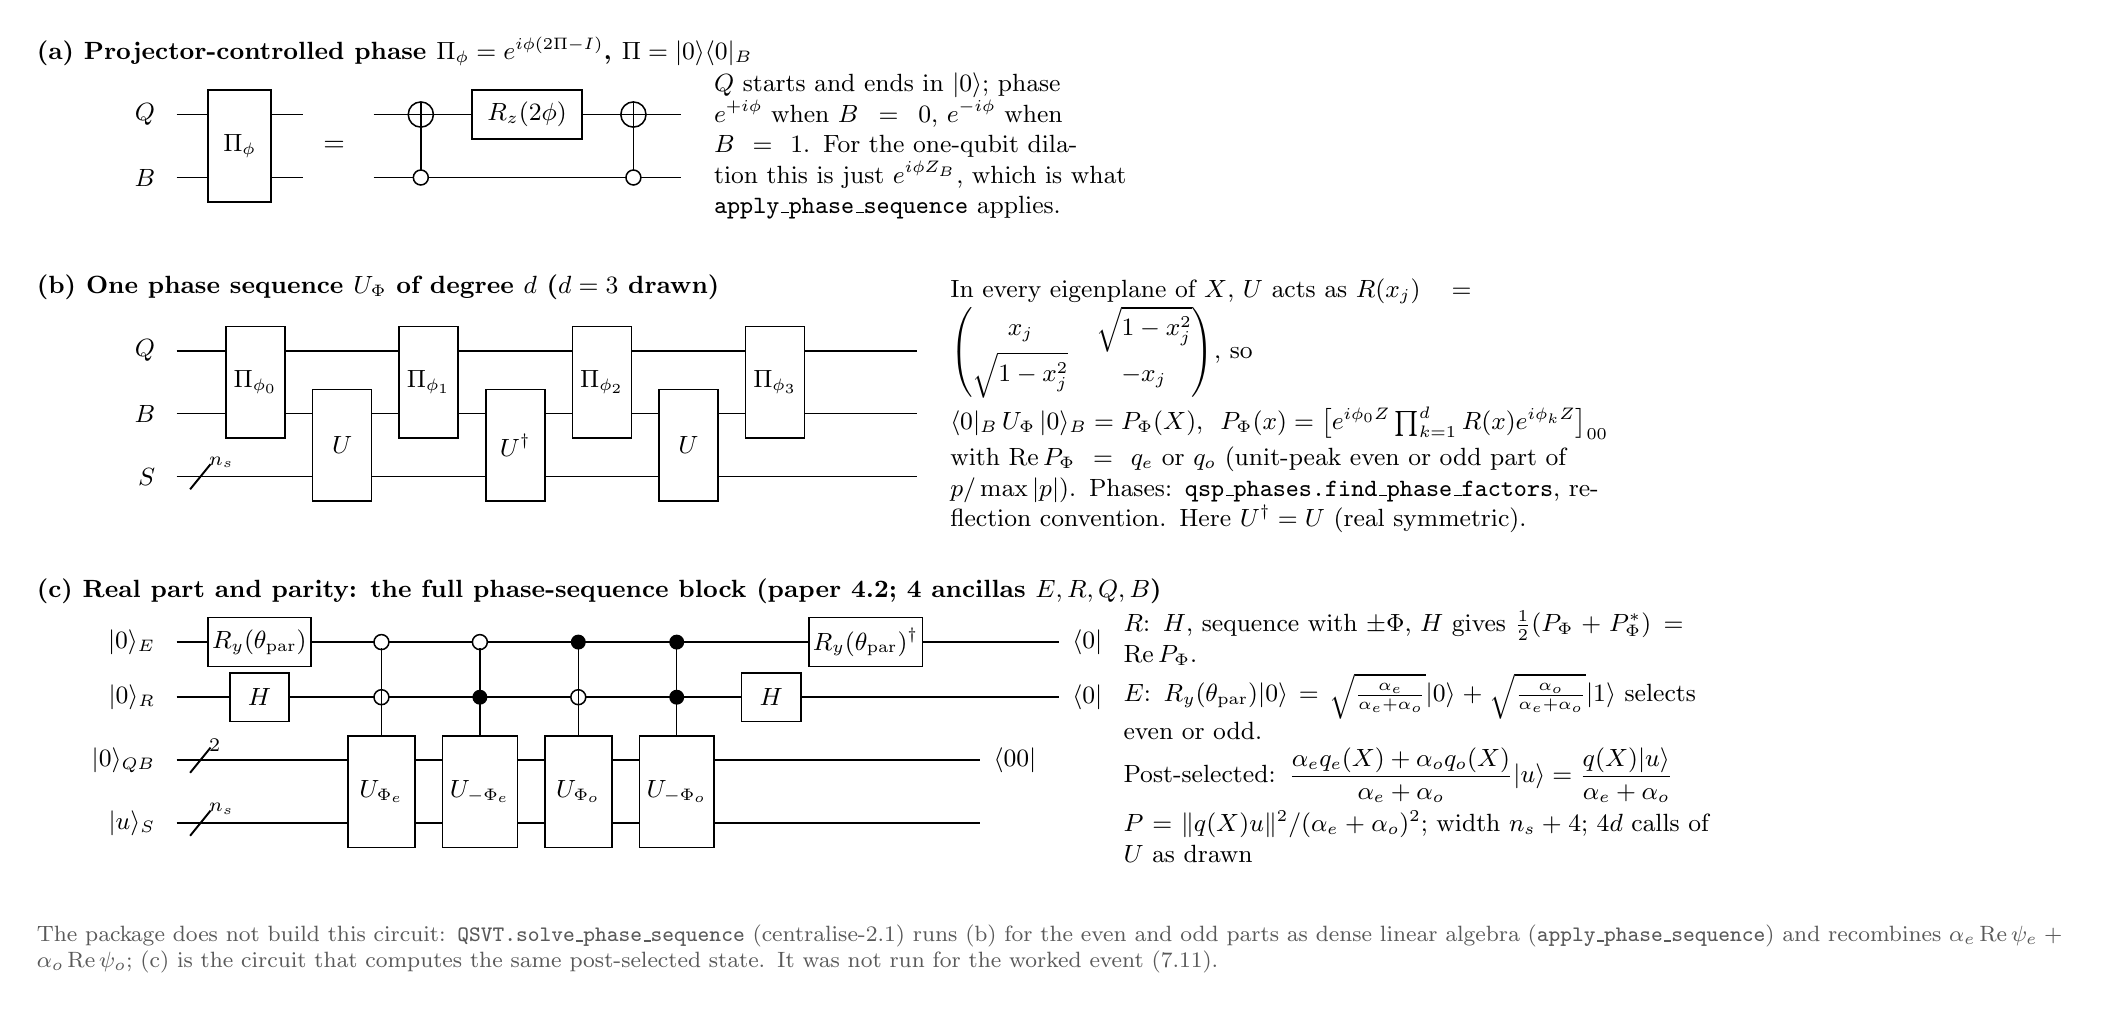
\begin{tikzpicture}[x=1cm,y=1cm]
% (a) projector-controlled phase
\node[anchor=west,font=\small\bfseries] at (-1.9,1.2) {(a) Projector-controlled phase $\Pi_\phi=e^{i\phi(2\Pi-I)}$, $\Pi=|0\rangle\langle0|_B$};
\lab{-0.15}{0.4}{$Q$} \lab{-0.15}{-0.4}{$B$}
\wires{0}{1.6}{0.4,-0.4}
\mb{0.8}{0.4}{-0.4}{0.8}{$\Pi_\phi$}
\node at (2.0,0) {$=$};
\wires{2.5}{6.4}{0.4,-0.4}
\oc{3.1}{-0.4} \vl{3.1}{-0.32}{0.4} \tg{3.1}{0.4}
\wg{4.45}{0.4}{14mm}{$R_z(2\phi)$}
\oc{5.8}{-0.4} \vl{5.8}{-0.32}{0.4} \tg{5.8}{0.4}
\node[font=\small,anchor=west,text width=5.6cm,align=left] at (6.7,0) {$Q$ starts and ends in $|0\rangle$; phase $e^{+i\phi}$ when $B=0$, $e^{-i\phi}$ when $B=1$. For the one-qubit dilation this is just $e^{i\phi Z_B}$, which is what \texttt{apply\_phase\_sequence} applies.};
% (b) one sequence
\begin{scope}[shift={(0,-3.0)}]
\node[anchor=west,font=\small\bfseries] at (-1.9,1.2) {(b) One phase sequence $U_\Phi$ of degree $d$ ($d=3$ drawn)};
\lab{-0.15}{0.4}{$Q$} \lab{-0.15}{-0.4}{$B$} \lab{-0.15}{-1.2}{$S$}
\wires{0}{9.4}{0.4,-0.4,-1.2} \slashwire{0.3}{-1.2}{$n_s$}
\mb{1.0}{0.4}{-0.4}{0.75}{$\Pi_{\phi_0}$}
\mb{2.1}{-0.4}{-1.2}{0.75}{$U$}
\mb{3.2}{0.4}{-0.4}{0.75}{$\Pi_{\phi_1}$}
\mb{4.3}{-0.4}{-1.2}{0.75}{$U^\dagger$}
\mb{5.4}{0.4}{-0.4}{0.75}{$\Pi_{\phi_2}$}
\mb{6.5}{-0.4}{-1.2}{0.75}{$U$}
\mb{7.6}{0.4}{-0.4}{0.75}{$\Pi_{\phi_3}$}
\node[font=\small,anchor=west,text width=8.8cm,align=left] at (9.7,-0.3) {In every eigenplane of $X$, $U$ acts as $R(x_j)=\begin{pmatrix}x_j&\sqrt{1-x_j^2}\\ \sqrt{1-x_j^2}&-x_j\end{pmatrix}$, so\\[2pt] $\langle0|_B\,U_\Phi\,|0\rangle_B=P_\Phi(X)$, \ $P_\Phi(x)=\big[e^{i\phi_0Z}\textstyle\prod_{k=1}^{d}R(x)e^{i\phi_kZ}\big]_{00}$\\[2pt] with $\mathrm{Re}\,P_\Phi=q_e$ or $q_o$ (unit-peak even or odd part of $p/\max|p|$). Phases: \texttt{qsp\_phases.find\_phase\_factors}, reflection convention. Here $U^\dagger=U$ (real symmetric).};
\end{scope}
% (c) real part and parity
\begin{scope}[shift={(0,-7.4)}]
\node[anchor=west,font=\small\bfseries] at (-1.9,1.75) {(c) Real part and parity: the full phase-sequence block (paper 4.2; 4 ancillas $E,R,Q,B$)};
\lab{-0.15}{1.1}{$|0\rangle_E$} \lab{-0.15}{0.4}{$|0\rangle_R$} \lab{-0.15}{-0.4}{$|0\rangle_{QB}$} \lab{-0.15}{-1.2}{$|u\rangle_S$}
\wires{0}{11.2}{1.1,0.4} \wires{0}{10.2}{-0.4,-1.2} \slashwire{0.3}{-0.4}{$2$} \slashwire{0.3}{-1.2}{$n_s$}
\wg{1.05}{1.1}{12mm}{$R_y(\theta_{\rm par})$} \gt{1.05}{0.4}{$H$}
% four controlled sequences
\oc{2.6}{1.1} \oc{2.6}{0.4} \vl{2.6}{1.02}{-0.4} \mb{2.6}{-0.4}{-1.2}{0.85}{$U_{\Phi_e}$}
\oc{3.85}{1.1} \ct{3.85}{0.4} \vl{3.85}{1.02}{-0.4} \mb{3.85}{-0.4}{-1.2}{0.95}{$U_{-\Phi_e}$}
\ct{5.1}{1.1} \oc{5.1}{0.4} \vl{5.1}{1.1}{-0.4} \mb{5.1}{-0.4}{-1.2}{0.85}{$U_{\Phi_o}$}
\ct{6.35}{1.1} \ct{6.35}{0.4} \vl{6.35}{1.1}{-0.4} \mb{6.35}{-0.4}{-1.2}{0.95}{$U_{-\Phi_o}$}
\gt{7.55}{0.4}{$H$} \wg{8.75}{1.1}{13mm}{$R_y(\theta_{\rm par})^\dagger$}
\node[font=\small,anchor=west] at (11.25,1.1) {$\langle0|$}; \node[font=\small,anchor=west] at (11.25,0.4) {$\langle0|$}; \node[font=\small,anchor=west] at (10.25,-0.4) {$\langle00|$};
\node[font=\small,anchor=west,text width=7.6cm,align=left] at (11.9,-0.1) {$R$: $H$, sequence with $\pm\Phi$, $H$ gives $\tfrac12(P_\Phi+P_\Phi^{*})=\mathrm{Re}\,P_\Phi$.\\[2pt] $E$: $R_y(\theta_{\rm par})|0\rangle=\sqrt{\tfrac{\alpha_e}{\alpha_e+\alpha_o}}|0\rangle+\sqrt{\tfrac{\alpha_o}{\alpha_e+\alpha_o}}|1\rangle$ selects even or odd.\\[2pt] Post-selected: $\dfrac{\alpha_eq_e(X)+\alpha_oq_o(X)}{\alpha_e+\alpha_o}|u\rangle=\dfrac{q(X)|u\rangle}{\alpha_e+\alpha_o}$\\[2pt] $P=\lVert q(X)u\rVert^2/(\alpha_e+\alpha_o)^2$; width $n_s+4$; $4d$ calls of $U$ as drawn};
\end{scope}
\node[font=\footnotesize,anchor=west,text=black!65,text width=26cm] at (-1.9,-10.2) {The package does not build this circuit: \texttt{QSVT.solve\_phase\_sequence} (centralise-2.1) runs (b) for the even and odd parts as dense linear algebra (\texttt{apply\_phase\_sequence}) and recombines $\alpha_e\,\mathrm{Re}\,\psi_e+\alpha_o\,\mathrm{Re}\,\psi_o$; (c) is the circuit that computes the same post-selected state. It was not run for the worked event (7.11).};
\end{tikzpicture}
\end{document}
